% Options for packages loaded elsewhere
\PassOptionsToPackage{unicode}{hyperref}
\PassOptionsToPackage{hyphens}{url}
%
\documentclass[
]{article}
\usepackage{lmodern}
\usepackage{amssymb,amsmath}
\usepackage{ifxetex,ifluatex}
\ifnum 0\ifxetex 1\fi\ifluatex 1\fi=0 % if pdftex
  \usepackage[T1]{fontenc}
  \usepackage[utf8]{inputenc}
  \usepackage{textcomp} % provide euro and other symbols
\else % if luatex or xetex
  \usepackage{unicode-math}
  \defaultfontfeatures{Scale=MatchLowercase}
  \defaultfontfeatures[\rmfamily]{Ligatures=TeX,Scale=1}
\fi
% Use upquote if available, for straight quotes in verbatim environments
\IfFileExists{upquote.sty}{\usepackage{upquote}}{}
\IfFileExists{microtype.sty}{% use microtype if available
  \usepackage[]{microtype}
  \UseMicrotypeSet[protrusion]{basicmath} % disable protrusion for tt fonts
}{}
\makeatletter
\@ifundefined{KOMAClassName}{% if non-KOMA class
  \IfFileExists{parskip.sty}{%
    \usepackage{parskip}
  }{% else
    \setlength{\parindent}{0pt}
    \setlength{\parskip}{6pt plus 2pt minus 1pt}}
}{% if KOMA class
  \KOMAoptions{parskip=half}}
\makeatother
\usepackage{xcolor}
\IfFileExists{xurl.sty}{\usepackage{xurl}}{} % add URL line breaks if available
\IfFileExists{bookmark.sty}{\usepackage{bookmark}}{\usepackage{hyperref}}
\hypersetup{
  pdftitle={Predicting diabetes mellitus using multiple correspondence analysis and machine learning},
  pdfauthor={Collin Hoskins},
  hidelinks,
  pdfcreator={LaTeX via pandoc}}
\urlstyle{same} % disable monospaced font for URLs
\usepackage[margin=1in]{geometry}
\usepackage{color}
\usepackage{fancyvrb}
\newcommand{\VerbBar}{|}
\newcommand{\VERB}{\Verb[commandchars=\\\{\}]}
\DefineVerbatimEnvironment{Highlighting}{Verbatim}{commandchars=\\\{\}}
% Add ',fontsize=\small' for more characters per line
\usepackage{framed}
\definecolor{shadecolor}{RGB}{248,248,248}
\newenvironment{Shaded}{\begin{snugshade}}{\end{snugshade}}
\newcommand{\AlertTok}[1]{\textcolor[rgb]{0.94,0.16,0.16}{#1}}
\newcommand{\AnnotationTok}[1]{\textcolor[rgb]{0.56,0.35,0.01}{\textbf{\textit{#1}}}}
\newcommand{\AttributeTok}[1]{\textcolor[rgb]{0.77,0.63,0.00}{#1}}
\newcommand{\BaseNTok}[1]{\textcolor[rgb]{0.00,0.00,0.81}{#1}}
\newcommand{\BuiltInTok}[1]{#1}
\newcommand{\CharTok}[1]{\textcolor[rgb]{0.31,0.60,0.02}{#1}}
\newcommand{\CommentTok}[1]{\textcolor[rgb]{0.56,0.35,0.01}{\textit{#1}}}
\newcommand{\CommentVarTok}[1]{\textcolor[rgb]{0.56,0.35,0.01}{\textbf{\textit{#1}}}}
\newcommand{\ConstantTok}[1]{\textcolor[rgb]{0.00,0.00,0.00}{#1}}
\newcommand{\ControlFlowTok}[1]{\textcolor[rgb]{0.13,0.29,0.53}{\textbf{#1}}}
\newcommand{\DataTypeTok}[1]{\textcolor[rgb]{0.13,0.29,0.53}{#1}}
\newcommand{\DecValTok}[1]{\textcolor[rgb]{0.00,0.00,0.81}{#1}}
\newcommand{\DocumentationTok}[1]{\textcolor[rgb]{0.56,0.35,0.01}{\textbf{\textit{#1}}}}
\newcommand{\ErrorTok}[1]{\textcolor[rgb]{0.64,0.00,0.00}{\textbf{#1}}}
\newcommand{\ExtensionTok}[1]{#1}
\newcommand{\FloatTok}[1]{\textcolor[rgb]{0.00,0.00,0.81}{#1}}
\newcommand{\FunctionTok}[1]{\textcolor[rgb]{0.00,0.00,0.00}{#1}}
\newcommand{\ImportTok}[1]{#1}
\newcommand{\InformationTok}[1]{\textcolor[rgb]{0.56,0.35,0.01}{\textbf{\textit{#1}}}}
\newcommand{\KeywordTok}[1]{\textcolor[rgb]{0.13,0.29,0.53}{\textbf{#1}}}
\newcommand{\NormalTok}[1]{#1}
\newcommand{\OperatorTok}[1]{\textcolor[rgb]{0.81,0.36,0.00}{\textbf{#1}}}
\newcommand{\OtherTok}[1]{\textcolor[rgb]{0.56,0.35,0.01}{#1}}
\newcommand{\PreprocessorTok}[1]{\textcolor[rgb]{0.56,0.35,0.01}{\textit{#1}}}
\newcommand{\RegionMarkerTok}[1]{#1}
\newcommand{\SpecialCharTok}[1]{\textcolor[rgb]{0.00,0.00,0.00}{#1}}
\newcommand{\SpecialStringTok}[1]{\textcolor[rgb]{0.31,0.60,0.02}{#1}}
\newcommand{\StringTok}[1]{\textcolor[rgb]{0.31,0.60,0.02}{#1}}
\newcommand{\VariableTok}[1]{\textcolor[rgb]{0.00,0.00,0.00}{#1}}
\newcommand{\VerbatimStringTok}[1]{\textcolor[rgb]{0.31,0.60,0.02}{#1}}
\newcommand{\WarningTok}[1]{\textcolor[rgb]{0.56,0.35,0.01}{\textbf{\textit{#1}}}}
\usepackage{graphicx}
\makeatletter
\def\maxwidth{\ifdim\Gin@nat@width>\linewidth\linewidth\else\Gin@nat@width\fi}
\def\maxheight{\ifdim\Gin@nat@height>\textheight\textheight\else\Gin@nat@height\fi}
\makeatother
% Scale images if necessary, so that they will not overflow the page
% margins by default, and it is still possible to overwrite the defaults
% using explicit options in \includegraphics[width, height, ...]{}
\setkeys{Gin}{width=\maxwidth,height=\maxheight,keepaspectratio}
% Set default figure placement to htbp
\makeatletter
\def\fps@figure{htbp}
\makeatother
\setlength{\emergencystretch}{3em} % prevent overfull lines
\providecommand{\tightlist}{%
  \setlength{\itemsep}{0pt}\setlength{\parskip}{0pt}}
\setcounter{secnumdepth}{-\maxdimen} % remove section numbering
\ifluatex
  \usepackage{selnolig}  % disable illegal ligatures
\fi

\title{Predicting diabetes mellitus using multiple correspondence
analysis and machine learning}
\author{Collin Hoskins}
\date{}

\begin{document}
\maketitle
\begin{abstract}
Machine learning provides many benefits to analyses of health
conditions. Machine learning models have been rapidly improving and will
continue to improve as more, unbiased data are available to build the
improved models. In this brief analysis and study, I measured the
performance of three machine learning algorithms in predicting diabetes
mellitus in individuals based on multiple predictor variables. The data
were split into a training and testing set in a 70/30 split (70\% of
observations fell in the training set, and 30\% of observations fell in
the testing set), which is typically the standard for machine learning. I
obtained the dataset from the University of California-Irvine Machine
Learning Repository (UCIMLR). The data are from direct interviews with
patients at Sylhet Diabetes Hospital in Sylhet, Bangladesh. The dataset
consists of 520 observations with 17 features (1 numerical, 16
categorical). The numerical feature (age), was converted into an age
group feature. Eight features were chosen to train the machine learning
models. These features were chosen based on results from a Multiple
Correspondence Analysis (MCA) on the data. The selected features were
used to train the following models: Logistic Regression, Support Vector
Machine Classification, Random Forest Classification, and Naive Bayes
Classification. The Random Forest Classification provided the lowest
prediction error (5.13\%). This model was also cross-validated using the
non-exhaustive K-fold Cross-Validation method which provided an
accuracy of 95\%. All analyses and data preprocessing were completed
using The R Project for Statistical Computing (R).
\end{abstract}

\hypertarget{introduction}{%
\section{Introduction}\label{introduction}}

Diabetes continues to become increasingly prevalent across different
ages and different demographics. In 2018, approximately 10.5\% of the
adult population of the United States had diabetes{[}1{]}. As the
prevalance continues to increase, the rate of undetection is also
increasing. Of the estimated 34.2 million adults with diabetes in 2018,
7.3 million were undiagonised {[}1{]}. The need for efficient and
accurate predictive models will continue to grow as artificial
intelligence (AI) in general, can be helpful in healthcare
decision-making{[}2{]}. Aside from the obvious health issues associated
with diabetes and the increased risk of death, those diagnosed with
diabetes have medical expenditures 2.3 times (2018 data) those without
diabetes. The total cost of diabetes in the United States in 2018 was
\$327 billion{[}1{]}. Machine learning can address what symptoms can
predict diabetes diagnoses, but it cannot address how to reduce the
overall prevalance of diabetes. It is clear that certain lifestyle
choices and habits can either decrease or increase the risk of developing
diabetes at any age{[}3{]}.

\hypertarget{objectives}{%
\section{Objectives}\label{objectives}}

\begin{itemize}
\item
  Find the features that explain the most variance of the response
  variable
\item
  Use Logistic Regression, Support Vector Machine Classification, and
  Random Forest Classification as machine learning models
\item
  Find the best machine learning model by comparing test error rates
\item
  Develop a final model that can be used to help doctors predict
  diabetes without waiting for laboratory test results
\end{itemize}

\hypertarget{analysis-plan}{%
\section{Analysis Plan}\label{analysis-plan}}

\hypertarget{exploratory-data-analysis}{%
\subsection{Exploratory Data Analysis}\label{exploratory-data-analysis}}

Exploring this dataset is accomplished mainly through various bar charts
with multiple conditions. Since all but one variables are binary, bar
charts will provide the most insight because counting the instances of
each binary value for each variable provides an oversight of which
features have more weight than other features.

\hypertarget{data-analytics-methods}{%
\subsection{Data Analytics Methods}\label{data-analytics-methods}}

\textbf{Data preprocessing} must occur first in order to complete all
proceeding analysis steps. The dataset used in this analysis is already
very clean and structured. The only preprocessing that occurred was
converting the range of values for the age variable into a categorical
feature, in which the categories are ``Young'', ``Mid-Young'',
``MidAge'', ``Mid-Old'', and ``Old''.

A \textbf{Chi-squared test} is used in this analysis to find variables
associated with the observed cases of diabetes that occur due to chance.
The resulting p-values from the Chi-squared test indicates the null
hypothesis that no relationship exists between each variable and the
response variable (diabetes) is rejected, and therefore an association
between the variable and the response variable exists{[}4{]}.

\textbf{Multiple Correspondence Analysis (MCA)} is used to reduce the
dimensions of a feature space. More specifically, MCA transforms the
categorical data such that many binary columns for each categorical
variable in the feature space are created, and only one column is valued
at 1. This process increased the dimensions because each categorical
variable is matched with multiple of the columns that were created.
These values were used to calculate the \textbf{Eigenvalue}. For each
dimension, the Eigenvalues are corrected using various approaches, but
they are then used to calculate the explained interia (variance) in the
dataset{[}5{]}. Using the calculated interia, a metric known as the
\textbf{squared cosine} is used to explain the degree of association
between certain variables{[}6{]}.

After utilizing MCA, the best features for the machine learning models
are selected, and the dataset is divided into a training set and a
testing set. The machine learning models considered are \textbf{Support
Vector Machine (SVM) Classification}, \textbf{Logistic Regression},
\textbf{Random Forest (RF) Classification}, and \textbf{Naive Bayes (NB)
Classification}. The algorithms are trained on the training data, and
are tested on the testing data. The testing portion provides predicted
values, which can be compared with the actual values. A confusion matrix
is used to compare predicted values from both classification models with
the actual observed values. The confusion matrix is helpful because it
highlights the true positives, false negatives, false positives, and
true negatives from the model. Since logistic regression transforms the
results into probabilities, the confusion matrix was not used for
simplicity in this case.

After each model was formed and used to predict diabetes in individuals,
the test error is calculated for each model. The model with the lowest
test error was also cross-validated using \textbf{K-fold
Cross-Validation}. K-fold cross-validation is a non-exhaustive
cross-validation method that shuffles and resamples the data, so that
each iteration (fold) of the validation process is composed of equal
counts of data.

\textbf{Note:} RF classification generally does not require k-fold
cross-validation because the data are already reshuffled and resampled
during each tree split in the model. However, since a training and
testing set is used in this analysis, the k-fold cross-validation
further confirms the model chosen was the one with the greatest
accuracy.

\hypertarget{data-summary}{%
\subsection{Data Summary}\label{data-summary}}

The dataset used in this analysis has 16 binary variables and 1
numerical variable. The response variable in this dataset is Class, in
which the levels are ``Positive'' and ``Negative''. See Figure 1 below
for an overview of the dataset{[}7{]}.

\begin{figure}[h!]
\centering
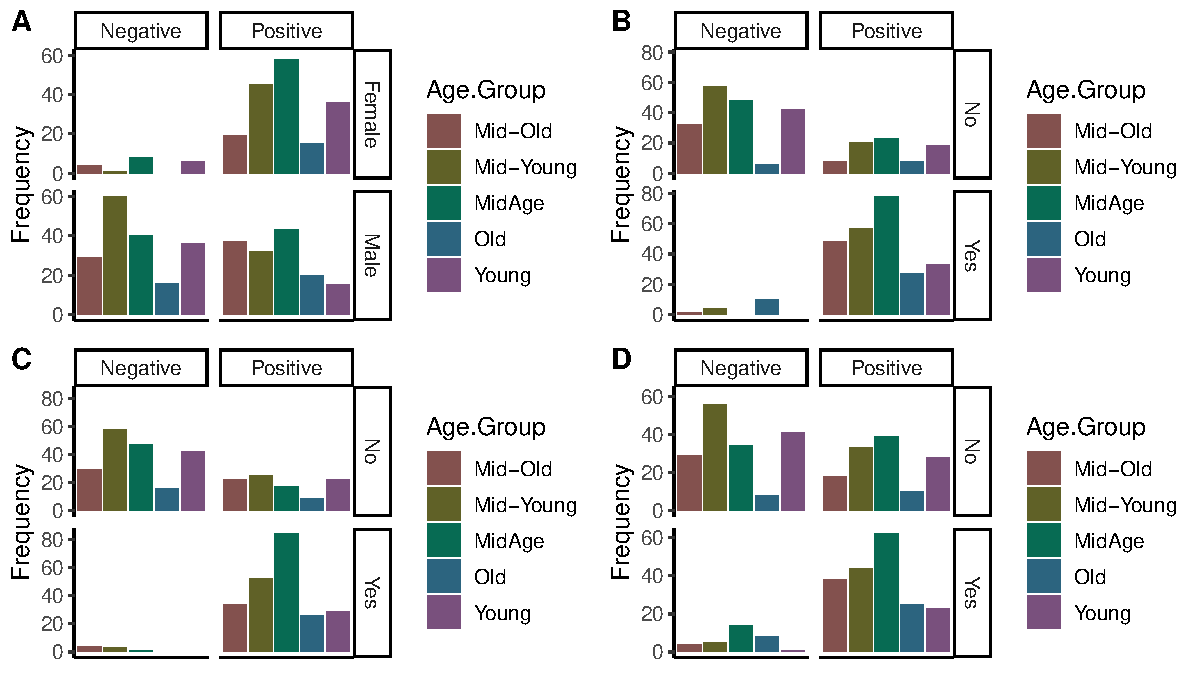
\includegraphics{FinalArticle_files/figure-latex/unnamed-chunk-2-1.pdf}
\caption{The Number of positive and negative counts for diabetes by age
group, as well as sex (A), Polyuria (B), Polydipsia (C), and Partial
Paresis (D).}
\end{figure}

The features that vary across subfigures Figure 1.B, Figure 1.C, and
Figure 1.D clearly occur more often in individuals of all ages who are
diagnosed positive for diabetes. Another important observation to note
is that those who do not have diabetes compose fewer counts than those
who tested positive and have the attribute. Also, notice difference
between counts of positive cases for those with polyuria (Figure 1.B)
and those with polydipsia (Figure 1.C).

\hypertarget{data-analysis-and-results}{%
\section{Data Analysis and Results}\label{data-analysis-and-results}}

\hypertarget{chi-squared-test}{%
\subsection{Chi-squared Test}\label{chi-squared-test}}

The Chi-squared test revealed that all features except Age group
(p.value = 0.12), Itching (p.value = 0.83), and Delayed Healing (p.value
= 0.33), do not occur due to chance alone. This gives a general idea of
some of the features that have more weight than others in their
associatiion with positive or negative diabetes cases. However, because
the machine learning models are most accurate when utilizing multiple
features, MCA is the best alternative to find the features most closely
associated other features.

\hypertarget{multiple-correspondence-analysis-mca}{%
\subsection{Multiple Correspondence Analysis
(MCA)}\label{multiple-correspondence-analysis-mca}}

Due to the size of the feature selection in this dataset (16), a
2-dimensional feature space is sufficient to find the most closely
related features (Figure 2.).

\begin{figure}[h!]
\centering
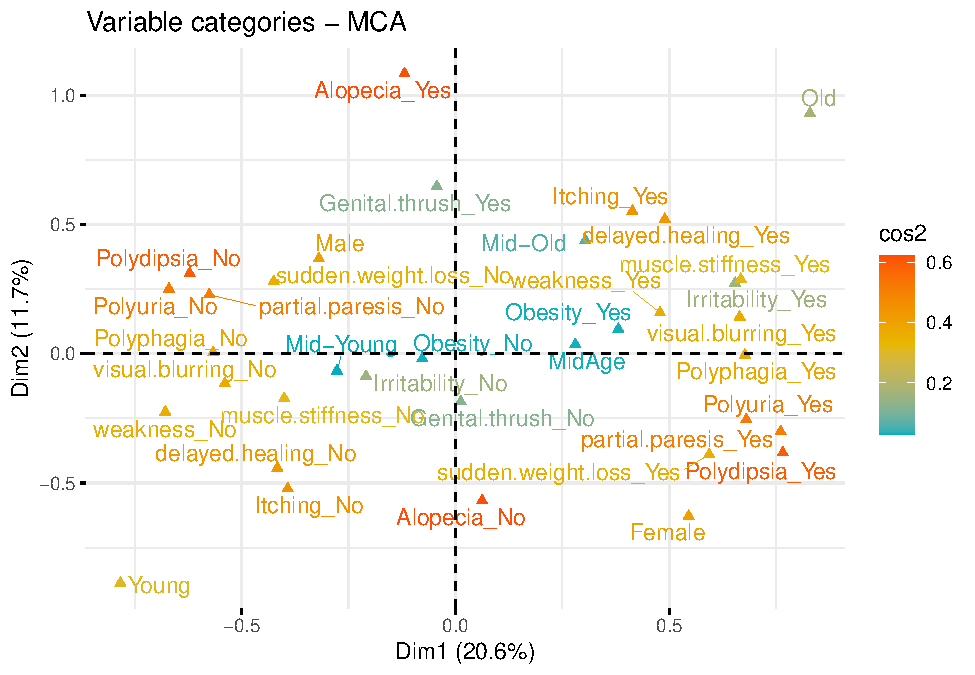
\includegraphics{FinalArticle_files/figure-latex/unnamed-chunk-3-1.pdf}
\caption{Visual representation of MCA.}
\end{figure}

The features chosen were selected by observing features with the
greatest cos2 value that all occur in dimension 1 (Dim1). The features
chosen were: \textbf{Polydipsia, Polyphagia, Partial Paresis, Polyuria,
Visual Blurring, Delayed Healing, Muscle Stiffness, and Gender.}

\hypertarget{splitting-the-dataset}{%
\subsection{Splitting the Dataset}\label{splitting-the-dataset}}

After the features were selected, subsamples of the dataset were
selected as the training set and the testing set. I decided to use the
stanard split ratio of 0.7. The training set consisted of 70\% of all
observations, and the testing set consisted of 30\% of all observations
(Table 1.).

\begin{table}[h!]

\caption{\label{tab:unnamed-chunk-4}Length of the training set and testing set.}
\centering
\begin{tabular}[t]{r|r}
\hline
Training & Testing\\
\hline
364 & 156\\
\hline
\end{tabular}
\end{table}

\hypertarget{machine-learning-algorithms}{%
\subsection{Machine Learning
Algorithms}\label{machine-learning-algorithms}}

Recall that logistic regression (LogReg), support vector machine (SVM)
classification, naive bayes (NB) classification, and random forest (RF) classification were used to find
the best predictive model. Logistic regression predicts the probability
of each observation in the testing set of having diabetes. The logistic
regression revealed many more counts of higher probabilities compared to
lower probabilities, but there were many counts near 0\% probability,
which indicates the model was successful in predicting negative cases of
diabetes as well (Figure 3.).

\begin{figure}[h!]
\centering
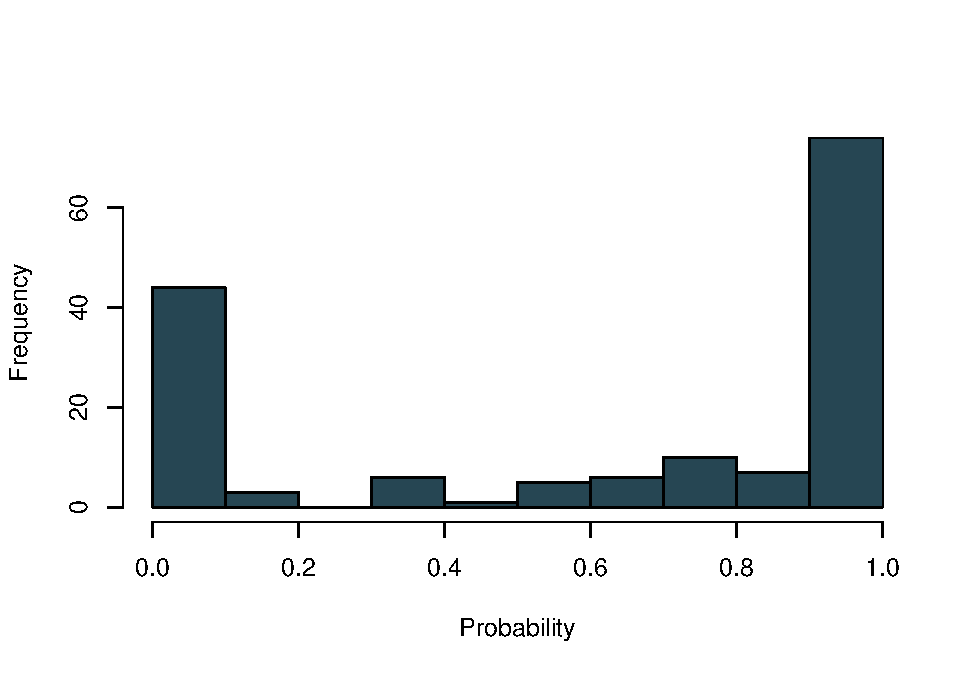
\includegraphics{FinalArticle_files/figure-latex/unnamed-chunk-6-1.pdf}
\caption{Frequency of probabilities produced from the logistic
regression on the testing set.}
\end{figure}

SVM classification and RF classification produce either ``Positive'' or
``Negative'' predictions for diabetes. These results can be compared to
the actual values from the testing set by using confusion matrices
(Figure 4.).

The bottom right corner of the confusion matrices indicate the true
positives. Notice how the SVM classification produced more true
positives than the RF classification, but the SVM classification also
produced many more false positives than the RF classification produced.
This increased the test error for SVM classification (Table 2.). Also,
the NB classification model produced false negatives, which increased
the test error for this model (Table 2.)

\begin{figure}[h!]
\centering
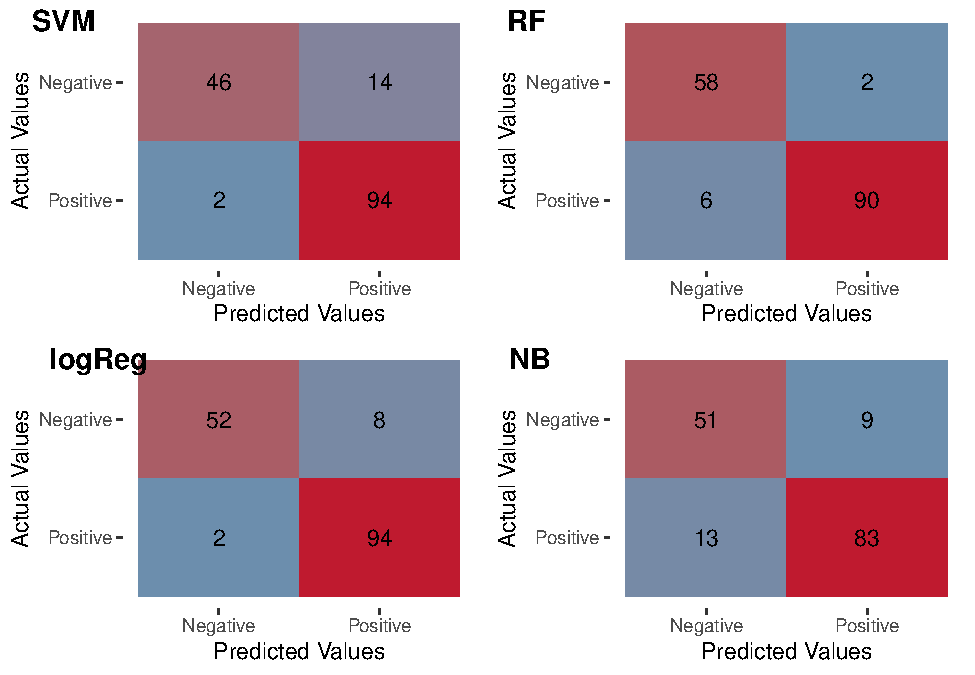
\includegraphics{FinalArticle_files/figure-latex/unnamed-chunk-11-1.pdf}
\caption{Confusion matrices comparing the actual and predicted values
for the support vector machine classification (SVM), random forest
classificaiton (RF), logistic regression (LogReg), and Naive Bayes
classification (NB).}
\end{figure}

The RF classification algorithm predicted the response variable with the
lowest test error of 5.13\%, compared to the logistic regression test
error of 6.41\%, and the SVM classification test error of 10.26\% (Table
2.). This indicates the RF classification model is the best model to use
to predict diabetes, based on the training dataset on which it was
trained. To further depict the accuracy of the model, K-fold
cross-validation was used to show the model accuracy across 10 different
folds (Table 3.).

\begin{table}[h!]

\caption{\label{tab:unnamed-chunk-12}Each Machine learning algorithm and the respective test error for each.}
\centering
\begin{tabular}[t]{l|r}
\hline
Test & Test Error\\
\hline
LogReg & 0.0641026\\
\hline
SVM & 0.1025641\\
\hline
RF & 0.0512821\\
\hline
NB & 0.1410256\\
\hline
\end{tabular}
\end{table}

\begin{table}[h!]

\caption{\label{tab:unnamed-chunk-14}Accuracy score from the 10-fold cross-validation RF classification.}
\centering
\begin{tabular}[t]{r}
\hline
Accuracy\\
\hline
0.949359\\
\hline
\end{tabular}
\end{table}

\hypertarget{discussion}{%
\section{Discussion}\label{discussion}}

As mentioned above, the test error for the random forest classification
was the lowest out of the three models. The low test error coupled with
the 10-fold cross-validation prove this machine learning algorithm was
the most effective out of the three chosen at prediciting diabetes
(Table 2.). This model could aid doctors in diagnosing diabetes prior to
receiving laboratory blood tests, which takes time. In a clinical setting
the random forest model could predict diabetes in indvididuals, but the
conditions for each feature in the model would have to be met, which is
not always the case.

The model could be improved by adding continous variables to the dataset
such as blood-glucose levels, etc. These variables would all likely be
derived from laboratory tests. In order to achieve this addition, a
newly formulated dataset is required. However, a new dataset with
continuous variables would likely increase the accuracy of the model, as
new feature selection techniques could be implemented, such as Principal
Component Analysis (PCA), which is very common among machine learning
practitioners.

For quick assessments, this model is sufficient in diagnosing diabetes.
It can, at the least, prompt those who likely have diabetes to undergo
blood work to officially receive a diabetes diagnosis. All research
objectives were met. However, as mentioned above, a better model can
always be constructed given a greater selection of attributes.

\hypertarget{conclusion}{%
\section{Conclusion}\label{conclusion}}

This analysis revealed the random forest classification is a sufficient
machine learning algorithm to predict diabetes mellitus in individuals.
The lack features available in the dataset used for analysis likely
reduced the performance of the model. However, this model is sufficient
at predicting diabetes mellitus about 95\% of the time. The predictive
power of this random forest model would increase given a dataset with
many more features, especially with the addition of continuous
laboratory-produced variables to the dataset.

\hypertarget{references}{%
\section{References}\label{references}}

\begin{itemize}
\item
  \emph{{[}1{]}:} Statistics About Diabetes \textbar{} ADA.
  Diabetes.org. (2018). Retrieved from
  \url{https://www.diabetes.org/resources/statistics/statistics-about-diabetes}.
\item
  \emph{{[}2{]}:} Signorini DF, Andrews PJD, Jones PA, et al Predicting
  survival using simple clinical variables: a case study in traumatic
  brain injuryJournal of Neurology, Neurosurgery \& Psychiatry
  (1999);66:20-25.
\item
  \emph{{[}3{]}:} Pnevmatikakis, Aristodemos, Stathis Kanavos, George
  Matikas, Konstantina Kostopoulou, Alfredo Cesario, and Sofoklis
  Kyriazakos. (2021). Risk Assessment for Personalized Health Insurance
  Based on Real-World Data.Risks 9: 46.
  \url{https://doi.org/10.3390/risks9030046}
\item
  \emph{{[}4{]}:} Ling.upenn.edu. (2008). Retrieved from
  \url{https://www.ling.upenn.edu/~clight/chisquared.htm}.
\item
  \emph{{[}5{]}:} Abdi, H., \& Valentin, D. (2015). Multiple
  Correspondence Analysis. Researchgate, 1,2,6,8. Retrieved from
  \url{https://www.researchgate.net/profile/Dominique-Valentin/publication/239542271_Multiple_Correspondence_Analysis/links/54a979900cf256bf8bb95c95/Multiple-Correspondence-Analysis.pdf}
\item
  \emph{{[}6{]}:} Essentials, M. (2021). MCA - Multiple Correspondence
  Analysis in R: Essentials - Articles - STHDA. Sthda.com. Retrieved
  from
  \url{http://www.sthda.com/english/articles/31-principal-component-methods-in-r-practical-guide/114-mca-multiple-correspondence-analysis-in-r-essentials/}.
\item
  \emph{{[}7{]}:} Islam, MM Faniqul, et al.~`Likelihood prediction of
  diabetes at early stage using data mining techniques.' Computer Vision
  and Machine Intelligence in Medical Image Analysis. Springer,
  Singapore, 2020. 113-125
\end{itemize}

\hypertarget{appendix}{%
\section{Appendix}\label{appendix}}

\hypertarget{r-code-used}{%
\subsection{R Code Used}\label{r-code-used}}

\begin{Shaded}
\begin{Highlighting}[]
\CommentTok{\# require(dplyr)}
\CommentTok{\# dataset \textless{}{-} read.csv("diabetes\_data\_upload.csv")}
\CommentTok{\# }
\CommentTok{\# dataset \textless{}{-} mutate(dataset, Age.Group = case\_when(Age \textless{}= 35 \textasciitilde{} "Young",}
\CommentTok{\#                                                  between(Age, 36, 45) \textasciitilde{} "Mid{-}Young",}
\CommentTok{\#                                                  between(Age, 46, 55) \textasciitilde{} "MidAge",}
\CommentTok{\#                                                  between(Age, 56, 65) \textasciitilde{} "Mid{-}Old",}
\CommentTok{\#                                                  Age \textgreater{}= 66 \textasciitilde{} "Old"))}
\CommentTok{\# dataset \textless{}{-} dataset[c("Gender", "Polyuria", "Polydipsia", "sudden.weight.loss", }
\CommentTok{\# "weakness", "Polyphagia", "Genital.thrush",}
\CommentTok{\# "visual.blurring", "Itching", "Irritability",}
\CommentTok{\# "delayed.healing", "partial.paresis", "muscle.stiffness",}
\CommentTok{\# "Alopecia", "Obesity", "Age.Group", "class")]}
\CommentTok{\# }
\CommentTok{\# }
\CommentTok{\# require(FactoMineR)}
\CommentTok{\# require(factoextra)}
\CommentTok{\# }
\CommentTok{\# }
\CommentTok{\# }
\CommentTok{\# }
\CommentTok{\# res.mca \textless{}{-} MCA(dataset[1:16], graph = F)}
\CommentTok{\# }
\CommentTok{\# fviz\_mca\_var(res.mca, col.var = "cos2",}
\CommentTok{\#              gradient.cols = c("\#00AFBB", "\#E7B800", "\#FC4E07"), }
\CommentTok{\#              repel = TRUE, \# Avoid text overlapping}
\CommentTok{\#              ggtheme = theme\_minimal())}
\CommentTok{\# }
\CommentTok{\# require(caTools)}
\CommentTok{\# }
\CommentTok{\# set.seed(101)}
\CommentTok{\# }
\CommentTok{\# sample \textless{}{-} sample.split(dataset$class, SplitRatio = 0.7)}
\CommentTok{\# }
\CommentTok{\# train \textless{}{-} subset(dataset, sample == TRUE)}
\CommentTok{\# }
\CommentTok{\# test \textless{}{-} subset(dataset, sample == FALSE)}
\CommentTok{\# }
\CommentTok{\# }
\CommentTok{\# trainSet \textless{}{-}select(train, Polydipsia, Polyphagia, partial.paresis, Polyuria, }
\CommentTok{\# visual.blurring, delayed.healing, muscle.stiffness, Gender, class)}
\CommentTok{\# }
\CommentTok{\# testSet \textless{}{-}  select(test, Polydipsia, Polyphagia, partial.paresis, Polyuria,}
\CommentTok{\# visual.blurring, delayed.healing, muscle.stiffness, Gender, class)}
\CommentTok{\# }
\CommentTok{\# descrData \textless{}{-} data.frame("Training" = length(trainSet[, 1]), }
\CommentTok{\# "Testing" = length(testSet[, 1]))}
\CommentTok{\# }
\CommentTok{\# require(kableExtra)}
\CommentTok{\# kbl(descrData, caption = "Length of the training set and testing set.")}
\CommentTok{\# }
\CommentTok{\# logReg \textless{}{-} glm(factor(class) \textasciitilde{} factor(Polydipsia)  + factor(Polyuria) + }
\CommentTok{\# factor(visual.blurring)}
\CommentTok{\# + factor(Polyphagia) + factor(partial.paresis) + }
\CommentTok{\# factor(delayed.healing) +}
\CommentTok{\#   factor(muscle.stiffness) + factor(Gender) ,}
  \CommentTok{\# family = binomial, data = trainSet)}
\CommentTok{\# }
\CommentTok{\# }
\CommentTok{\# }
\CommentTok{\# logPredict \textless{}{-} predict(logReg, testSet[{-}9], type = "response")}
\CommentTok{\# }
\CommentTok{\# hist(logPredict, main = NULL, xlab = "Probability", col = "\#264653")}
\CommentTok{\# }
\CommentTok{\# require(e1071)}
\CommentTok{\# }
\CommentTok{\# SVMClass \textless{}{-} svm(factor(class) \textasciitilde{} factor(Polydipsia)  + factor(Polyuria) +}
\CommentTok{\# factor(visual.blurring) + factor(Polyphagia) + factor(partial.paresis) + }
\CommentTok{\# factor(delayed.healing) +    factor(muscle.stiffness) + factor(Gender), }
\CommentTok{\# kernel = "linear", data = trainSet)}
\CommentTok{\# }
\CommentTok{\# SVMPredict \textless{}{-} predict(SVMClass, testSet[{-}9], type = "response")}
\CommentTok{\# }
\CommentTok{\# require(randomForest)}
\CommentTok{\# }
\CommentTok{\# RFClass \textless{}{-} randomForest(x = trainSet[{-}9], y = factor(trainSet$class), ntree = 20)}
\CommentTok{\# }
\CommentTok{\# RFPredict \textless{}{-} predict(RFClass, testSet[{-}9], type = "response")}


\CommentTok{\# require(e1071)}
\CommentTok{\# }
\CommentTok{\# }
\CommentTok{\# }
\CommentTok{\# NBClass \textless{}{-} naiveBayes(x = trainSet[{-}9], y = factor(trainSet$class))}
\CommentTok{\# }
\CommentTok{\# NBPredict \textless{}{-} predict(NBClass, testSet[{-}9])}

\CommentTok{\# }
\CommentTok{\# logYPred \textless{}{-} ifelse(logPredict \textgreater{} 0.5, "Positive", "Negative")}
\CommentTok{\# }
\CommentTok{\# logRegError \textless{}{-} 1 {-} mean(logYPred == testSet$class)}
\CommentTok{\# }
\CommentTok{\# SVMError \textless{}{-} 1 {-} mean(SVMPredict == testSet$class)}
\CommentTok{\# }
\CommentTok{\# RFError \textless{}{-} 1 {-} mean(RFPredict == testSet$class)}

\CommentTok{\# NBError \textless{}{-} 1 {-} mean(NBPredict == testSet$class)}

\CommentTok{\# }
\CommentTok{\# require(ggpubr)}
\CommentTok{\# require(yardstick)}
\CommentTok{\# }
\CommentTok{\# }
\CommentTok{\# Atemp \textless{}{-} conf\_mat(table(testSet[, 9], SVMPredict))}
\CommentTok{\# }
\CommentTok{\# Btemp \textless{}{-} conf\_mat(table(testSet[, 9], RFPredict))}
\CommentTok{\# }
\CommentTok{\# Ctemp \textless{}{-} conf\_mat(table(testSet[, 9], logYPred))}
\CommentTok{\# }
\CommentTok{\# Dtemp \textless{}{-} conf\_mat(table(testSet[, 9], NBPredict))}
\CommentTok{\# }
\CommentTok{\# }
\CommentTok{\# A \textless{}{-} autoplot(Atemp, type = "heatmap") + scale\_fill\_gradient(low = "\#6c8ead", }
\CommentTok{\#                                                              high = "\#bf1a2f")+}
\CommentTok{\# xlab("Predicted Values") }
\CommentTok{\# + ylab("Actual Values")}
\CommentTok{\# }
\CommentTok{\# B \textless{}{-} autoplot(Btemp, type = "heatmap") + scale\_fill\_gradient(low = "\#6c8ead", }
\CommentTok{\#                                                              high = "\#bf1a2f") + }
\CommentTok{\# xlab("Predicted Values") }
\CommentTok{\# + ylab("Actual Values")}
\CommentTok{\# }
\CommentTok{\# C \textless{}{-} autoplot(Ctemp, type = "heatmap") + scale\_fill\_gradient(low = "\#6c8ead",}
\CommentTok{\#                                                              high = "\#bf1a2f") +}
\CommentTok{\# xlab("Predicted Values") }
\CommentTok{\# + ylab("Actual Values")}
\CommentTok{\# }
\CommentTok{\# D \textless{}{-} autoplot(Dtemp, type = "heatmap") + scale\_fill\_gradient(low = "\#6c8ead", }
\CommentTok{\#                                                              high = "\#bf1a2f") +}
\CommentTok{\# xlab("Predicted Values") }
\CommentTok{\# + ylab("Actual Values")}
\CommentTok{\# }
\CommentTok{\# }
\CommentTok{\# ggarrange(A, B, C, D, labels = c("SVM", "RF", "logReg", "NB"), nrow = 2, ncol = 2)}
\CommentTok{\# }
\CommentTok{\# ggarrange(A, B, labels = c("SVM", "RF"))}
\CommentTok{\# }
\CommentTok{\# testErrorDf \textless{}{-} data.frame(Test \textless{}{-} c("LogReg", "SVM", "RF"),}
\CommentTok{\# Values \textless{}{-} c(logRegError, SVMError, RFError, NBError))}
\CommentTok{\# kbl(testErrorDf,}
\CommentTok{\# caption = "Each Machine learning algorithm and the respective test error for each.",}
\CommentTok{\#       col.names = c("Test", "Test Error"))}
\CommentTok{\# }
\CommentTok{\# require(caret)}
\CommentTok{\# }
\CommentTok{\# combTestTain \textless{}{-} rbind(trainSet, testSet)}
\CommentTok{\# }
\CommentTok{\# }
\CommentTok{\# train\_control \textless{}{-} trainControl(method = "cv", number = 10)}
\CommentTok{\# }
\CommentTok{\# RFcvModel \textless{}{-} train(factor(class) \textasciitilde{} ., data = combTestTain, method = "rf", }
\CommentTok{\# trControl = train\_control)}
\CommentTok{\# }
\CommentTok{\# kbl(data.frame(Accuracy = mean(RFcvModel$results[, 2])), }
\CommentTok{\# caption = "Accuracy score from the 10{-}fold cross{-}validation RF classification.")}
\end{Highlighting}
\end{Shaded}



\end{document}
